
\documentclass{standalone}
\usepackage{tikz}
\usepackage{xcolor}
\usepackage{amsmath}
\usepackage{varwidth}
\usepackage{pgfornament}
\usetikzlibrary{fit,shapes,positioning,backgrounds}
\newcommand{\magnitude}[1] {
    \ifnum #1 = 0
        ~
    \else
        \times 10^{#1}~
    \fi
}
\tikzset{
    namenode/.style={
        execute at begin node={\begin{varwidth}{45mm}\begin{center}},
        execute at end node={\end{center}\end{varwidth}},
    },
    formulaenode/.style={
        execute at begin node={\small $\textcolor{gray}},
        execute at end node={$},
    },
    valuenode/.style={
        execute at begin node={$},
        execute at end node={$},
    },
    symbolnode/.style={
        scale=2,
        execute at begin node={\Huge $},
        execute at end node={$},
    },
    diagsymbolnode/.style={
        execute at begin node={\Large $},
        execute at end node={$},
    },
}
\begin{document}
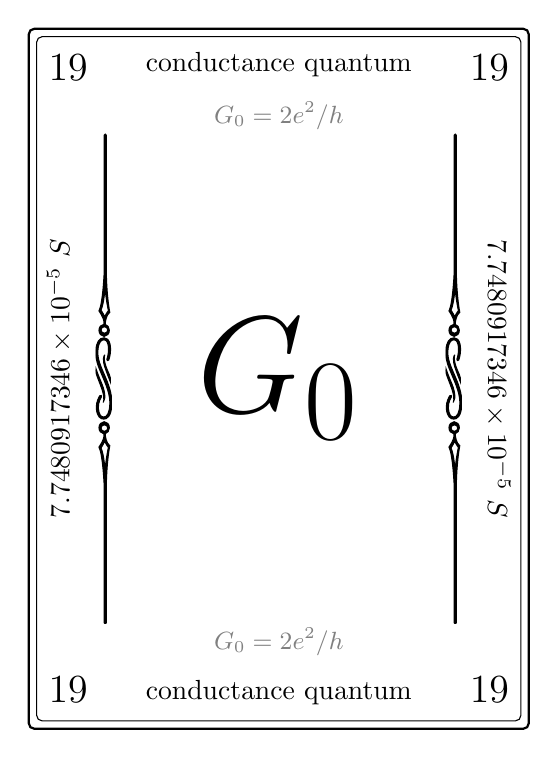
\begin{tikzpicture}[x=1mm,y=1mm]
    \def\w{63.5};
    \def\h{88.9};
    \def\k{5};

    \coordinate (north) at (0,0.5*\h);
    \coordinate (south) at (0,-0.5*\h);
    \coordinate (east) at (0.5*\w,0);
    \coordinate (west) at (-0.5*\w,0);

    \def\name{conductance quantum};
    \def\symbol{G_0};
    \def\formulae{G_0 = 2 e^2 / h};
    \def\value{7.7480917346};
    \def\power{-5};
    \def\unit{S};
    \def\order{19};

    \draw[thick,rounded corners=2pt] (-0.5*\w,-0.5*\h) rectangle (0.5*\w,0.5*\h);
    \draw[thin,rounded corners=2pt] (-0.5*\w+1,-0.5*\h+1) rectangle (0.5*\w-1,0.5*\h-1);

    \path (-0.35*\w,-0.35*\h) to [ornament=88] (-0.35*\w,0.35*\h);
    \path (0.35*\w,-0.35*\h) to [ornament=88] (0.35*\w,0.35*\h);

    \node[symbolnode] (C) at (0,0) {\symbol};
    \node[diagsymbolnode] (D1) at (0.5*\w-\k,-0.5*\h+\k) {\order};
    \node[diagsymbolnode] (D2) at (0.5*\w-\k,0.5*\h-\k) {\order};
    \node[diagsymbolnode] (D3) at (-0.5*\w+\k,-0.5*\h+\k) {\order};
    \node[diagsymbolnode] (D2) at (-0.5*\w+\k,0.5*\h-\k) {\order};

    \node[namenode,below = 5pt of north] (N1) {\name};
    \node[namenode,above = 5pt of south] (N2) {\name};

    \node[valuenode,right = 3pt of west,rotate=90,anchor=north] (V1) {\value\magnitude{\power}\unit};
    \node[valuenode,left = 3pt of east,rotate=-90,anchor=north] (V2) {\value\magnitude{\power}\unit};
    \node[formulaenode,below = 2pt of N1] (F1) {\formulae};
    \node[formulaenode,above = 2pt of N2] (F2) {\formulae};
\end{tikzpicture}
\end{document}
